\documentclass[letterpaper]{article}
\usepackage{amsmath}
\usepackage{geometry}
\usepackage[utf8]{inputenc}
\usepackage{listings}
\usepackage{minted}
\usepackage{hyperref}
\usepackage{xcolor}
\usepackage{graphicx}
\usepackage[shortlabels]{enumitem}
\usepackage[skip=12pt, indent=0pt]{parskip}
\usepackage{makecell}
\usepackage{tablefootnote}
\usepackage{pgfgantt}
\usepackage{wrapfig}
\usepackage{chngpage}


\geometry{letterpaper,left=1in,right=1in,top=1.0in,bottom=1.0in,headheight=28pt}

\definecolor{codegreen}{rgb}{0,0.6,0}
\definecolor{codegray}{rgb}{0.5,0.5,0.5}
\definecolor{codecrimson}{RGB}{153,0,0}
\definecolor{backcolour}{rgb}{0.95,0.95,0.92}
\makeatletter
\lstdefinestyle{mystyle}{
  backgroundcolor=\color{backcolour},   commentstyle=\color{codegreen},
  keywordstyle=\color{blue},
  numberstyle=\tiny\color{codegray},
  stringstyle=\color{codecrimson},
  basicstyle=\ttfamily,
  breakatwhitespace=false,         
  breaklines=true,                 
  captionpos=b,                    
  keepspaces=true,                 
  numbers=left,                    
  numbersep=5pt,                  
  showspaces=false,                
  showstringspaces=false,
  showtabs=false,                  
  tabsize=2
}
\makeatother
\lstset{style=mystyle}
\title{Thick Origami Kinematics Simulator}
\author{Jacob Pavelka, Anvay Pradhan, Noah Zambrano}
\date{November 2023}

\begin{document}
%%% Commenting Commands
\newcommand{\Jacob}[1]{{\normalsize{\textbf{({\color{blue} Jacob:\ }#1)}}}}
\newcommand{\Anvay}[1]{{\normalsize{\textbf{({\color{red} Anvay:\ }#1)}}}}
\newcommand{\Noah}[1]{{\normalsize{\textbf{({\color{green} Noah:\ }#1)}}}}

\maketitle

\section*{Background and Motivation}
\subsection*{Introduction}
Kinematic Simulation is an important tool for many problems. For linkage systems, it allows one to study the degrees of freedom of a system or its range of motion. For computer graphics, simulating kinematics is important for virtual reality training, video games, rapid digital prototyping, and robotics simulation \cite{SiggraphContact22}.
For structural systems it allows one to study whether or not a system is stable. For example, understanding the kinematic properties of thick origami is important if it is used structurally. A kinematic simulation would show which forces would cause the origami to deform without resistance \cite{filipov2015toward}. 

\textit{For our project, we want to develop a kinematic simulation package for thick, rigid origami so we can become more familiar with kinematic simulation methods and develop performant software that others can use.} To test our package, we will simulate kinematic folding motions for a simple hinge made of two objects, a Miura fold, and a cube folded from flat. This project will incorporate course themes including scripting, linear algebra and libraries, object-oriented programming (OOP), workflows, and unit testing.

\subsection*{Background}
The kinematics of an origami object can be simulated by first defining the origami's mesh based on pre-defined nodes, then imposing constraints on those nodes' degrees of freedom based on the defined mesh, and finally, solving for the mesh's kinematically admissible motion based on the constraints \cite{zhu2022review}. 
%
\begin{wrapfigure}[18]{o}{0.47\textwidth}
    \centering
    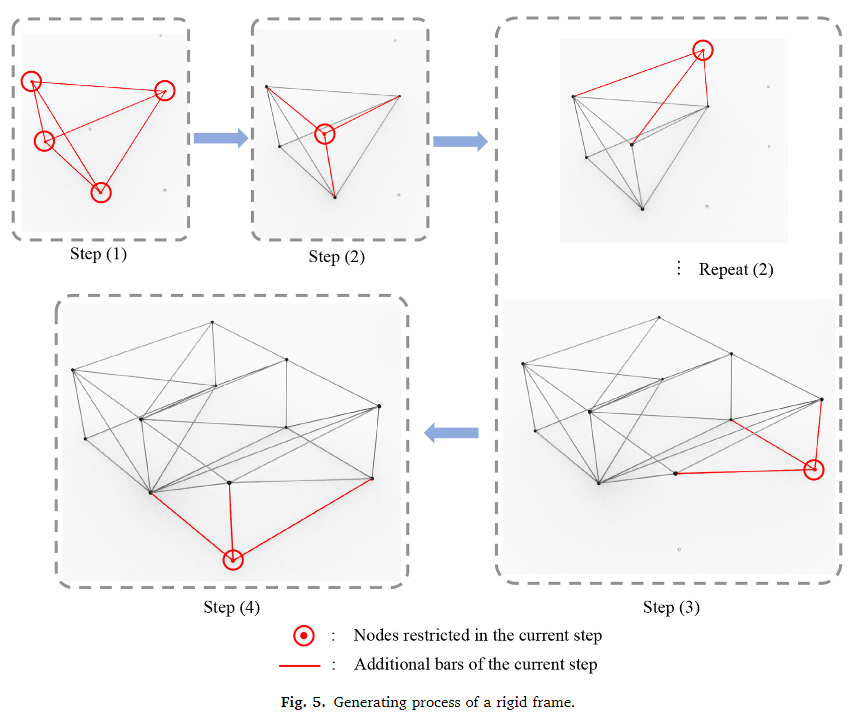
\includegraphics[width=0.47\columnwidth]{mesh_gen.png}
    \caption{Procedure for generating a mesh given predefined nodes \cite{zhang2021folding}.}
    \label{fig:mesh_gen}
\end{wrapfigure}
%
To simulate the kinematics of an object, it first needs to be represented mathematically, wich can be done by creating a mesh of the object. There are many methods for creating meshes, but we will use the one described in \cite{zhang2021folding} because it creates a mesh of edges and nodes that is automatically stable.

This algorithm begins with a list of nodes that describe the important features of a convex hull, such as any corners. From here, four nodes are chosen randomly such that they create a tetrahedron, and links are defined between them. Then, another point is chosen randomly and connected to three existing points such that they all form another tetrahedron. Links are created between the three existing nodes and the new node. This process is repeated for all remaining nodes. Figure \ref{fig:mesh_gen} illustrates this. This process will create the mesh for one rigid object, but to have objects that can develop complex motion, one or more objects will to be connected. This will be taken care of in later steps.

Once all points are connected, a connectivity matrix can be formed, and from this, the constraints can be formed. The general constraint that will be made for each connection is shown in Eq.~\ref{cosntraint}.
\begin{equation}
    l^2=(\Vec{x_i}-\Vec{x_j})\cdot (\Vec{x_i}-\Vec{x_j}) 
    \label{cosntraint}
\end{equation}
Where $x_i$ and $x_j$ are the position vectors of connected nodes, and $l$ is the original distance between the two nodes. 

Implementing this constraint ensures the distance between nodes remains constant to enforce rigid body kinematics. Compiling these constraints into one matrix and linearizing them with respect to time, a new relationship is defined in Eq.~\ref{linearized_cosntraint}. When this matrix is compiled, adjacent nodes of connected bodies should also be constrained by Eq.~\ref{cosntraint}

\begin{equation}
    0=C\dot x
    \label{linearized_cosntraint}
\end{equation}

Where $\dot x$ is a vector of each degree of freedom's velocity. 

This equation can be solved, but it has multiple solutions. A better approach to finding kinematically admissible velocities is to project a trial velocity vector onto the null space of the constraint matrix as shown in Eq.~\ref{Project}.
\begin{equation}
    \dot x=[I-C^+C]\dot x_0
    \label{Project}
\end{equation}


Ultimately, the goal of the simulator is to find the new node locations $x_{s+1}$ for each timestep in terms of the original node locations $x_s$ under applied loads. To do so, we can represent the new node locations in the following manner:
\begin{equation}
    x_{s+1}=x_s+dx_s
\end{equation}
where $dx_s$ is a vector of constraints linearized with respect to time to produce infinitesimal admissible motions (see Eq. \ref{Maclaurin}). These can be integrated over time to achieve the full motion. Many methods may be used to integrate the velocities and higher-order terms over time, but we will use Eq.~\ref{Maclaurin} in our implementation unless another is warranted.
\begin{equation}
    dx_s\approx \dot{x}dt+\ddot{x} \frac{dt^k}{k!}
    \label{Maclaurin}
\end{equation}

\section*{Tasks}
To develop this simulation software, we will incorporate github for collaboration, cmake to help build the project, and a waterfall development workflow, where we will define the requirements of the software, then its architecture, through the rest of the steps, and finish with testing. The architecture will be designed with the Object Oriented Programming paradigm and the unified modeling language. The actual software will be developed using C++ and will integrate any performant linear algebra or scientific computing packages needed (blas,lapack,petsc). Testing, visualization, and example cases will be developed for this software too, and the example cases will be ran on Great Lakes.

\begin{table}[H]
    \centering
    \caption{Tasks with Person In Charge, Descriptions, and Deliverables}
    \centerline{
    \begin{tabular}{|p{0.25cm}|p{4cm}|p{2.3cm}|p{6cm}|p{4cm}|}
    \hline
     \# & Task/Topic & PIC & Description & Deliverable  \\\hline
     
   1 & Github (Workflows)& Jacob & Update issues and review tasks, push code  & Completed and reviewed tasks, repo link \\\hline
   
     2 &Code Architecture (C++ OOP)& Jacob  & Develop code structure by defining classes  & UML diagram \\\hline
     
     3 & Set up project file structure and compilation tools (CMAKE, Tools of the Trade) & Anvay  & Define a storage system for the elements of the software and begin making the tools to configure,build, and install the software, where the remaining portions of the cmake tools will be defined as the code is developed & Project File structure developed and initial programs compile \\\hline

     4 & Integrate Linear Algebra or Scientific Computing Libraries (Linear Algebra and Libraries)& Noah &Link linear algebra library (e.g. openBLAS) to aid in linear algebra operations, specifically the matrix solve and matrix-operations & Functioning code that successfully utilizes library \\\hline
     
     5 & Meshing Implementation (C++ OOP)& Jacob & Write code to generate mesh from input file containing points of interest on convex hull. Update CMAKE, github with changes. & Functioning code that passes tests \\\hline
     
     6 & Define Constraints (C++ OOP)& Noah & Implement methods to generate the constraint matrix. Update CMAKE, github with changes. & Functioning code that passes tests \\\hline
     
     7 & Kinematics Implementation (C++ OOP)& Anvay & Implement methods to compute kinematically admissible deformations. Update CMAKE, github with changes. & Functioning code that passes tests \\\hline

     8 & Unit Testing, Verification Testing, and Examples (Workflows/C++ OOP/Great lakes)& Noah & Write tests for each method, run required tests and example cases on Great Lakes, and confirm results are correct & At least one test is defined for every method and they all pass \\\hline
     
     9 & Visualization (Scripting)& Anvay & Implement a python script to produce animations of the simulation & Video files that can be included in our presentation\\\hline
     
     10 & Presentation& All & Write slides for presentation  & Powerpoint file \\\hline
     
     11 & Report& All & Write sections of report  &  Completed report PDF and links to repo\\\hline
    \end{tabular}
    }
\end{table}


\section*{Estimated Schedule}

\definecolor{barblue}{RGB}{153,204,254}
\definecolor{groupblue}{RGB}{51,102,254}
\definecolor{linkred}{RGB}{165,0,33}
\renewcommand\sfdefault{phv}
\renewcommand\mddefault{mc}
\renewcommand\bfdefault{bc}
\setganttlinklabel{s-s}{START-TO-START}
\setganttlinklabel{f-s}{FINISH-TO-START}
\setganttlinklabel{f-f}{FINISH-TO-FINISH}
\sffamily
\begin{ganttchart}[
    canvas/.append style={fill=none, draw=black!5, line width=.75pt},
    hgrid style/.style={draw=black!5, line width=.75pt},
    vgrid={*1{draw=black!5, line width=.75pt}},
    today=1, % update today line here
    today rule/.style={
      draw=black!64,
      dash pattern=on 3.5pt off 4.5pt,
      line width=1.5pt
    },
    today label font=\small\bfseries,
    title/.style={draw=none, fill=none},
    title label font=\bfseries\footnotesize,
    title label node/.append style={below=7pt},
    include title in canvas=false,
    bar label font=\mdseries\small\color{black!70},
    bar label node/.append style={left=2cm},
    bar/.append style={draw=none, fill=black!63},
    bar incomplete/.append style={fill=barblue},
    bar progress label font=\mdseries\footnotesize\color{black!70},
    group incomplete/.append style={fill=groupblue},
    group left shift=0,
    group right shift=0,
    group height=.5,
    group peaks tip position=0,
    group label node/.append style={left=.6cm},
    group progress label font=\bfseries\small,
    link/.style={-latex, line width=1.5pt, linkred},
    link label font=\scriptsize\bfseries,
    link label node/.append style={below left=-2pt and 0pt}
  ]{1}{13}
  \gantttitle[
    title label node/.append style={below left=7pt and -3pt}
  ]{WEEKS:\quad1}{2}
  \gantttitlelist{2,...,7}{2} \\
  % \ganttgroup[progress=0]{Noah's Tasks}{4}{8} \\
  \ganttbar[ name=T1]{\textbf{Task 1} Github - Jacob}{2}{5} \\
  \ganttbar[ name=T2]{\textbf{Task 2} Project Architecture - Jacob}{2}{3} \\
  \ganttbar[ name=T1]{\textbf{Task 3} Project Files Structure and CMAKE - Anvay}{2}{5} \\
  \ganttbar[
    name=T4
  ]{\textbf{Task 4} Libraries - Noah}{4}{7} \\
  \ganttbar[ name=T5]{\textbf{Task 5} Meshing Implementation - Jacob}{4}{8} \\
  \ganttbar[
    name=T6
  ]{\textbf{Task 6} Constraint Matrix - Noah}{4}{8} \\
  \ganttbar[ name=T4]{\textbf{Task 7} Kinematic iterator - Anvay}{4}{8} \\
  \ganttbar[
    name=T8
  ]{\textbf{Task 8} Unit Tests - Noah}{4}{8} \\[grid]
  % \ganttgroup[progress=0]{Jacob's Tasks}{4}{10} \\
  % \ganttgroup[progress=0]{Anvay's Tasks}{4}{10} \\
  \ganttbar[]{\textbf{Task 9} Visualization - Anvay}{9}{9} \\
  \ganttbar[]{\textbf{Task 10} Presentation - All}{2}{9} \\
  \ganttbar[]{\textbf{Task 11} Report - All}{2}{13} \\
  % \ganttlink[link type=s-s]{T2}{T3}
  % \ganttlink[link type=f-s]{T3}{T7}
  %\ganttlink[
   % link type=f-f,
   % link label node/.append style=left
 % ]{T3}{T7}
\end{ganttchart}


\bibliographystyle{plain}
\bibliography{refs}
\end{document}

\end{document}
